\documentclass[conference]{IEEEtran}
\IEEEoverridecommandlockouts

% The preceding line is only needed to identify funding in the first footnote. If that is unneeded, please comment it out.
\usepackage{cite}
\usepackage{amsmath,amssymb,amsfonts}
%\usepackage{algorithmic}
\usepackage[]{algorithm2e}
\usepackage{graphicx}
\usepackage{textcomp}
\usepackage{xcolor}
\usepackage{lipsum}

\usepackage[]{siunitx}

\bibliographystyle{IEEEtran}

% Enumerations
\usepackage[inline]{enumitem}
\renewcommand*\descriptionlabel[1]{\hspace\labelsep\itshape #1}

% Spacing
\usepackage{xspace}

% Tables
\usepackage{booktabs}
\usepackage{multirow}
\newcommand{\specialcell}[3][c]
{\begin{tabular}[#1]{@{}#2@{}}#3\end{tabular}}

% Acronyms
\usepackage[acronym,nowarn]{glossaries}
\glsdisablehyper
%==============================================================================
% Institutions 
%=============================================================================

% PUC Minas
\newacronym{pucminas}{PUC Minas}{Pontifícia Universidade Católica de Minas Gerais}
	\newcommand{\pucminas}{\gls{pucminas}\xspace}

% UFSC
\newacronym{ufsc}{UFSC}{Universidade Federal de Santa Catarina}
	\newcommand{\ufsc}{\gls{ufsc}\xspace}

% UGA
\newacronym{uga}{UGA}{Univerité Grenoble Alpes}
	\newcommand{\uga}{\gls{uga}\xspace}

% Grenoble INP
\newacronym{inpg}{Grenoble INP}{Institut National Polytechnique de Grenoble}
	\newcommand{\inpg}{\gls{inpg}\xspace}

%==============================================================================
% Computer Architecture
%=============================================================================

% Manycores
\newcommand{\scc}{Intel Single-Cloud Computer\xspace}
\newcommand{\xeonphi}{Intel Xeon Phi\xspace}
\newcommand{\tilegx}{Tilera TILE-Gx100\xspace}
\newcommand{\tilepro}{Tilera TILE64\xspace}
\newcommand{\mppa}{Kalray MPPA-256\xspace}
\newcommand{\pulp}{PULP\xspace}
\newcommand{\taihulight}{Sunway SW26010\xspace}
\newcommand{\epiphany}{Adapteva Epiphany\xspace}
\newcommand{\optimsoc}{OpTiMSoC\xspace}
\newcommand{\hero}{HERO\xspace}
\newcommand{\celerity}{Celerity\xspace}

% Architecture Families
\newcommand{\amd}{x86-64\xspace}
\newcommand{\intel}{x86\xspace}
\newcommand{\openrisc}{OpenRISC\xspace}
\newcommand{\bostan}{Bostan\xspace}
\newcommand{\riscv}{RISC-V\xspace}

% ISA
\newacronym{isa}{ISA}{Instruction Set Architecture}
	\newcommand{\isa}{\gls{isa}\xspace}

% FIFO
\newacronym{fifo}{FIFO}{First-In First-Out}
	\newcommand{\fifo}{\gls{fifo}\xspace}

% VLIW
\newacronym{vliw}{VLIW}{Very Long Instruction Word}
	\newcommand{\vliw}{\gls{vliw}\xspace}

% Taxonomy
\newacronym{mimd}{MIMD}{Multiple Instruction Multiple Data}
	\newcommand{\mimd}{\gls{mimd}\xspace}
\newacronym{simd}{SIMD}{Single Instruction Multiple Data}
	\newcommand{\simd}{\gls{simd}\xspace}
\newacronym{numa}{NUMA}{Non-Uniform Memory Access}
	\newcommand{\numa}{\gls{numa}\xspace}
\newacronym{norma}{NoRMA}{No Remote Memory Access}
	\newcommand{\norma}{\gls{norma}\xspace}
\newacronym{amp}{AMP}{Asymmetric Multi-Processing}
	\newcommand{\amp}{\gls{amp}\xspace}
\newacronym{smp}{SMP}{Symmetric Multi-Processing}
	\newcommand{\smp}{\gls{smp}\xspace}
\newacronym{gpu}{GPU}{Graphics Processing Unit}
	\newcommand{\gpu}{\gls{gpu}\xspace}
	\newcommand{\gpus}{\glspl{gpu}\xspace}
\newacronym{fpga}{FPGA}{Field Programmable Gate Array}
	\newcommand{\fpga}{\gls{fpga}\xspace}
	\newcommand{\fpgas}{\glspl{fpga}\xspace}

% Core
\newacronym{pe}{PE}{Processing Element}
	\newcommand{\pe}{\gls{pe}\xspace}
	\newcommand{\pes}{\glspl{pe}\xspace}
\newacronym{rm}{RM}{Resource Manager}
	\newcommand{\rman}{\gls{rm}\xspace}
	\newcommand{\rmans}{\glspl{rm}\xspace}

\newcommand{\iocluster}{I/O Cluster\xspace}
\newcommand{\ioclusters}{I/O Clusters\xspace}
\newcommand{\ccluster}{Compute Cluster\xspace}
\newcommand{\cclusters}{Compute Clusters\xspace}

\newcommand{\cluster}{\textit{cluster}\xspace}
\newcommand{\clusters}{\textit{clusters}\xspace}

\newcommand{\microkernel}{\textit{microkernel}\xspace}
\newcommand{\multikernel}{\textit{multikernel}\xspace}

\newcommand{\lw}{\textit{lightweight manycore}\xspace}
\newcommand{\lws}{\textit{lightweight manycores}\xspace}

% MMU
\newacronym{mmu}{MMU}{Memory Management Unit}
	\newcommand{\mmu}{\gls{mmu}\xspace}
	\newcommand{\mmus}{\glspl{mmu}\xspace}

% Cache
\newcommand{\dcache}{d-cache\xspace}
\newcommand{\icache}{i-cache\xspace}

\newacronym{raw}{RaW}{Read after Write}
	\newcommand{\raw}{\gls{raw}\xspace}

% TLB
\newacronym{tlb}{TLB}{Translation Lookaside Buffer}
	\newcommand{\tlb}{\gls{tlb}\xspace}
	\newcommand{\tlbs}{\glspl{tlb}\xspace}

% J-TLB
\newacronym{jtlb}{JTLB}{Join TLB}
	\newcommand{\jtlb}{\gls{jtlb}\xspace}
	\newcommand{\jtlbs}{\gls{jtlb}\xspace}

% L-TLB
\newacronym{ltlb}{LTLB}{Locked TLB}
	\newcommand{\ltlb}{\gls{ltlb}\xspace}
	\newcommand{\ltlbs}{\glspl{ltlb}\xspace}

% I-TLB
\newacronym{itlb}{ITLB}{Instruction TLB}
	\newcommand{\itlb}{\gls{itlb}\xspace}

% D-TLB
\newacronym{dtlb}{DTLB}{Data TLB}
	\newcommand{\dtlb}{\gls{dtlb}\xspace}

% SRAM
\newacronym{sram}{SRAM}{Static Random Access Memory}
	\newcommand{\sram}{SRAM\xspace}

% DRAM
\newacronym{dram}{DRAM}{Dynamic Random Access Memory}
	\newcommand{\dram}{DRAM\xspace}

% SPD
\newacronym[plural=SPMs,firstplural=Scratchpad Memories (SPMs)]{spm}{SPM}{Scratchpad Memory}
	\newcommand{\spm}{\gls{spd}\xspace}
	\newcommand{\spms}{\glspl{spm}\xspace}

% DMA
\newacronym{dma}{DMA}{Direct Memory Access}
	\newcommand{\dma}{\gls{dma}\xspace}

% RMA
\newacronym{rma}{RMA}{Remote Memory Access}
	\newcommand{\rma}{\gls{rma}\xspace}

% NoC
\newacronym[plural=NoCs,firstplural=Redes-em-Chip (NoCs)]{noc}{NoC}{Rede-em-Chip}
	\newcommand{\noc}{\gls{noc}\xspace}
	\newcommand{\nocs}{\glspl{noc}\xspace}

% C-NoC
\newacronym{cnoc}{C-NoC}{Control NoC}
    \newcommand{\cnoc}{\gls{cnoc}\xspace}

% D-NoC
\newacronym{dnoc}{D-NoC}{Data NoC}
	\newcommand{\dnoc}{\gls{dnoc}\xspace}

%==============================================================================
% Operating Systems
%=============================================================================

% OS
\newacronym{os}{OS}{Sistema Operacional}
\newacronym[plural=OSes,firstplural=Sistemas Operacionais (OSes)]{os}{OS}{Sistema Operacional}
	\newcommand{\os}{\gls{os}\xspace}
	\newcommand{\oses}{\glspl{os}\xspace}

% POSIX
\newacronym{posix}{POSIX}{Portable Operating System Interface}
	\newcommand{\posix}{\gls{posix}\xspace}

% Kernels
\newcommand{\barrelfish}{Barrelfish\xspace}
\newcommand{\linux}{Linux\xspace}
\newcommand{\unix}{Unix\xspace}
\newcommand{\rtems}{RTEMS\xspace}
\newcommand{\bsd}{BSD\xspace}
\newcommand{\nodeos}{NodeOS\xspace}
\newcommand{\nanvix}{Nanvix\xspace}
\newcommand{\mossca}{MOSSCA\xspace}
\newcommand{\popcorn}{Popcorn Linux\xspace}
\newcommand{\helios}{Helios\xspace}
\newcommand{\tessellation}{Tessellation\xspace}
\newacronym{lfour}{L4}{L4 Microkernel}
	\newcommand{\lfour}{\gls{lfour}\xspace}

% Operating Systems
\newcommand{\gnu}{GNU/Linux\xspace}
\newacronym{fos}{FOS}{Factored Operating System}
	\newcommand{\fos}{\gls{fos}\xspace}
\newacronym{nos}{nOS}{Nano-Sized Operating System}
	\newcommand{\nos}{\gls{nos}\xspace}

% HAL
\newacronym{hal}{HAL}{Camada de Abstração de Hardware}
	\newcommand{\hal}{\gls{hal}\xspace}
	\newcommand{\hals}{\glspl{hal}\xspace}

% API
\newacronym{api}{API}{Application Programming Interface}
	\newcommand{\api}{\gls{api}\xspace}
	\newcommand{\apis}{\glspl{api}\xspace}

% IPC
\newacronym{ipc}{IPC}{Inter-Process Communication}
	\newcommand{\ipc}{\gls{ipc}\xspace}

% COM
\newacronym{com}{COM}{Communication}
	\newcommand{\com}{\gls{com}\xspace}

% RMem
\newacronym{rmem}{RMem}{Remote Memory}
	\newcommand{\rmem}{\gls{rmem}\xspace}

% QoS
\newacronym{qos}{QoS}{Quality of Service}
	\newcommand{\qos}{\gls{qos}\xspace}

% RPC
\newacronym{rpc}{RPC}{Remote Producere Call}
	\newcommand{\rpc}{\gls{rpc}\xspace}


%==============================================================================
% High Performance Computing
%=============================================================================

% HPC
\newacronym{hpc}{HPC}{High-Performance Computing}
	\newcommand{\hpc}{\gls{hpc}\xspace}

% OpenMP
\newcommand{\openmp}{OpenMP}\xspace
\newcommand{\javaconcurrency}{Java Concurrency\xspace}
\newcommand{\pthreads}{POSIX Threads}\xspace
\newcommand{\tbb}{TBB}\xspace
\newcommand{\cilk}{Cilk}\xspace

% PGAS
\newacronym{pgas}{PGAS}{Partitioned Global Address Space}
	\newcommand{\pgas}{\gls{pgas}\xspace}
\newacronym{mpi}{MPI}{Message Passing Interface}
	\newcommand{\mpi}{\gls{mpi}\xspace}

%==============================================================================
% Other
%=============================================================================

\newcommand{\ie}{i.e.\xspace}
\newcommand{\eg}{e.g.\xspace}
\newcommand{\etal}{\textit{et al.}\xspace}

\newacronym{iid}{i.i.d}{Independent and Identically Distributed}
	\newcommand{\iid}{\gls{iid}\xspace}

\newacronym{anova}{ANOVA}{Analysis of Variance}
	\newcommand{\anova}{\gls{anova}\xspace}

%==============================================================================
% Benchmarks 
%=============================================================================


\newcommand{\microbenchmark}{\si{\micro}benchmark\xspace}
\newcommand{\Microbenchmark}{\si{\micro}Benchmark\xspace}
\newcommand{\microbenchmarks}{\si{\micro}benchmarks\xspace}
\newcommand{\Microbenchmarks}{\si{\micro}Benchmarks\xspace}

% Local Kernel Call
\newacronym{lkcall}{L-Kcall}{Local Kernel Call}
	\newcommand{\lkcall}{\gls{lkcall}\xspace}

% Remote Kernel Call
\newacronym{rkcall}{R-Kcall}{Remote Kernel Call}
	\newcommand{\rkcall}{\gls{rkcall}\xspace}

% Upcall
\newcommand{\upcall}{Upcall\xspace}

% Fork-Join
\newcommand{\forkjoin}{ForkJoin\xspace}

% Producer-Consumer
\newcommand{\buffer}{Buffer\xspace}

% Gaussian Filter
\newacronym{knoise}{KNoise}{Kernel Noise}
	\newcommand{\knoise}{\gls{knoise}\xspace}

\newcommand{\sync}{\textit{sync}\xspace}
\newcommand{\mailbox}{\textit{mailbox}\xspace}
\newcommand{\portal}{\textit{portal}\xspace}



\makeglossaries

% Bookmarks.
\usepackage{xcolor}
\usepackage[bookmarks,bookmarksopen,bookmarksdepth=2,colorlinks=true]{hyperref}
\hypersetup{
	citecolor   = blue,
	linkcolor   = blue,
	urlcolor    = blue,
    pdftitle    = { On the performance and Isolation of Asymmetric
	                Microkernel Design for Lightweight Manycores },
    pdfauthor   = {Pedro Henrique Penna},
    pdfcreator  = {Pedro Henrique Penna},
    pdfproducer = {Pedro Henrique Penna},
    pdfsubject  = {Operating Systems},
}

\linespread{0.95}

% Images
\usepackage{graphicx}
\graphicspath{{img/}}
\DeclareGraphicsExtensions{.pdf,.jpeg,.png}

% Review
\usepackage{todonotes}
\usepackage{lipsum}

\hyphenation{Kal-ray}
\hyphenation{light-weight}
\hyphenation{as-sess-es}

\def\BibTeX{{\rm B\kern-.05em{\sc i\kern-.025em b}\kern-.08em
    T\kern-.1667em\lower.7ex\hbox{E}\kern-.125emX}}

\linespread{0.95}

\begin{document}

\title{
	OS-Level Task-Based Mechanism for Lightweight Manycore Processors
}

\author{%
	\IEEEauthorblockN{João Vicente Souto}
	\IEEEauthorblockA{%
		\textit{UFSC}\\
		Florianópolis, Brazil\\
		joao.vicente.souto@grad.ufsc.br
	}
	\and
	\IEEEauthorblockN{Pedro Henrique Penna}
	\IEEEauthorblockA{%
		\textit{UGA, PUC Minas}\\
		Grenbole, France\\
		pedro.penna@sga.pucminas.br
	}
	\and
	\IEEEauthorblockN{Márcio Castro}
	\IEEEauthorblockA{%
		\textit{UFSC}\\
		Florianópolis, Brazil\\
		marcio.castro@ufsc.br
	}
}

\maketitle

	
\begin{abstract}
	Lightweight manycore processors stand out for their high level of
	parallelism and energy efficiency. However, its architectural
	characteristics introduce several challenges in software development. One
	of the central difficulties is the limited amount of local memory that the
	applications have available to work. This limitation needs to be considered
	by software solutions for \lws. In this context, this work proposes the
	definition of a task mechanism within an asymmetric microkernel designed
	for \lws. This mechanism makes it possible to define multiple execution
	streams at a low cost to the memory system through the implementation of
	a limited number of special threads. The results showed that the proposed
	mechanism achieved similar performance to that of a dedicated thread to
	each task.
\end{abstract}

\begin{IEEEkeywords}
	HAL, Distributed Operating System, Lightweight Manycore, Kalray MPPA-256
\end{IEEEkeywords}

	\section{Introduction}
\label{sec:introduction}

	% Context
	A classe de processadores Lightweight Manycore destaca-se pela seu alto
	nível de paralelismo com baíxo consumo energético~\cite{francesquini2015}. As
	aplicações projetadas para executar nesses processadores tem a sua disposição
	centenas de núcleos agrupados e distribuídos em um único chip. Para endereçar
	a escalabilidade do sistema e prover a eficiência energética, LWs exibem
	características arquiteturais próprias que os diferem dos demais Manycores.
	Especificamente, eles integram:
	\begin{enumerate*}[label=(\roman*)]
		\item thousands of low-power cores with \mimd capability~\cite{Rossi2017};

		\item distributed memory architecture and small local memories shared by
			tightly-coupled groups of cores (aka \textit{clusters})~\cite{Bohnenstiehl2017};

		\item reliable and fast \nocs for message-passing~\cite{Bohnenstiehl2017}; and

		\item heterogeneous processing capabilities~\cite{Davidson2018}.
	\end{enumerate*}
	Alguns exemplos de LWs são A, B e C.

\iffalse
	%
	Esses processadores introduziram junto de suas vantagens, um conjunto de
	desafios no projeto e desenvolvimento de aplicações de baíxo e alto nível
	inserido pelas suas características arquiteturais. Algumas desses desafios
	são:
	\begin{itemize}
		\item Modelo de Programação Híbrida: uso do modelo de memória
			compartilhada para explorar o paralelismo dentro dos clusters e
			aplicação do modelo de troca de mensagens para lidar com
			comunicação entre clusters através da NoC~\cite{kelly2013};

		\item Falta de suporte em hardware para coerência de cache: para
			reduzir o consumo de energia requirindo o controle explícito da
			memória~\cite{francesquini2015};.

		\item Sistem de memória restritivo: a presença de múltiplos espaços de
			endereçamento e pequenas memórias locais requer o Data Tiling
			e Prefetching seja manipulado em software~\cite{Castro2016};

		\item Configurações heterogeneas: requer a programação de componentes
			distintos, dificultando o deploy de aplicações no
			LWs~\cite{Barbalace2015}.
	\end{itemize}
\fi

	% Motivation
	Tais características introduzem diversos desafios no desenvolvimento de
	aplicações de baíxo e alto nível. Por exemplo, 
	\begin{enumerate*}[label=(\roman*)]
		\item programação híbrida entre os modelos de memória compartilhada
			e troca de mensagens devido a natureza dos LWs~\cite{kelly2013};

		\item falta de suporte em hardware para coerência de
			cache\cite{francesquini2015};

		\item sistema de memória distribuído e restritivo~\cite{Castro2016}; e 

		\item programação de componentes heterogêneos~\cite{Barbalace2015}.
	\end{enumerate*}
	Neste contexto, diversos trabalhos propõem soluções em diversos níveis de
	abstração para amenizar as dificuldades e prover ao usuário final
	alternativas para o desenvolvimento dessas arquiteturas.
	%
	Soluções em nível do kernel, como PENNA-NANVIX, endereçam uma gama de
	problemas de baíxo nível para prover uma visão padronizada e facilitar
	a programabilidade e portabilidade para LWs.
	%
	Por outro lado, soluções como XXX, buscam em explorar um tipo específico de
	abstração e modelaam um esqueleto de solução que pode ser adaptado pra
	família de problemas endereçado.

	% Problem Definition
	Dentre todas as soluções, uma das principais dificuldades é como lidar
	com a quantidade reduzida de memória local dentro de um cluster. Vale
	ressaltar que essa memória muitas vezes não é exclusiva para o usuário.
	A memória local precisa armazenar códigos e estruturas de  dados da
	aplicação e de suas dependências, e.g., OS e/ou bibliotecas.
	Algo que consome uma quantidade considerável de memória é o suporte
	a múltiplos fluxos de programação. Por exemplo, alocação de páginas de
	memória para armazenar o contexto e pilha de execução de uma rotina.
	%
	% Goals and Contributions
	Neste contexto, o presente trabalho propõe uma abstração de task em nível
	de kernel para definir uma unidade genérica de execução. Similar a uma
	piscina de threads, uma thread do sistema aguarda receber essas unidades
	para executar.
	Com este mecanismo, buscamos atingir os seguintes objetivos
	e contribuíções:
	\begin{itemize}
		\item Projetar um mecanismo de task no nível do kernel para uso interno
			do OS e para a aplicação cliente.

		\item Diminuir a alocação de memória do sistema de threads ao
			reutilizar o contexto e pilha de execução de uma única thread;

		\item Melhorar a utilização de núcleos ociosos;

		\item Explorar a localidade dos dados na cache de um único núcleo;

		\item Habilitar operações assíncrona e/ou periódicas, e.g.,
			envio assíncrono em LWs que não possuem DMA.

		\item Facilitar a modelagem de funcionalidades internas do kernel.
	\end{itemize}
	Este trabalho faz parte do desenvolvimento do Nanvix, um sistema operacional
	distribuído projetado para endereçar as características dos LWs. O escopo
	do trabalho se limita ao aperfeiçoamento do um microkernel assimétrico que
	gerencia os recursos locais de um cluster.

	% Work Organization
	The remainder of this work is organized as follows.
	In Section~\ref{sec:related-work}, we discuss related work.
	In Section~\ref{sec:problem} we cover the problem definition.
	In Section~\ref{sec:solution}, we present our proposal.
	In Section~\ref{sec:platform}, we detail the experimental environment.
	In Section~\ref{sec:results}, we discuss our experimental results.
	In Section~\ref{sec:related-work} we discuss related works.
	In Section~\ref{sec:conclusions}, we draw our conclusions.

	\section{Related Work}
\label{sec:related-work}

	\lipsum[2-4]

	\section{Problem Definition}
\label{sec:problem}

	% Overview
	O gerenciamento de memória interna de um cluster afeta todos os níveis de
	abstração no contexto dos LWs. Por exemplos, OSs precisam ser pequenos
	e leves para deixar a maior quantidade de memória disponível pra aplicação.
	Por outro lado, aplicações extremamente paralelas e concorrentes têm
	a necessidade de gerenciar manualmente a coerência dos dados manipulados.

	Para amenizar os problemas de coerência de
	cache existente nessas arquiteturas, Penna ETAL propôs um microkernel
	assímetrico para concentrar o gerenciamento e manipulação das estruturas do
	OS em um único núcleo. A Figura X ilustra a execução de uma chamada de
	sistema dentro do Nanvix. Quando um núcleo escravo deseja realizar uma operação
	privilegiada, este envia uma solicitação ao núcleo mestre, que por sua vez,
	realiza e retorna o resultado ao solicitante. Os problemas explorados neste
	trabalho estão contidos no escopo deste nível de OS.

	Além das dificuldades impostas pelo sistema de memória, nossa proposta
	busca atacar algumas das desvantagens do microkernel e do sistema de
	comunicação. As descrições a seguir sumarizam os principais problemas que nossa
	solução se propõe endereçar:

	% Problems
	\begin{description}

		\item[Memory Utilizationg] Para cada novo fluxo de execução (thread),
			o sistema de memória deve reservar dois espaços de memória, um
			para a pilha de execução do usuário e outra reservada para
			o kernel. Geralmente, cada pilha possúi o tamanho de uma página de
			memória, crescendo rapidamente a quantidade de memória necessária
			para criar novas threads no sistema.

		\item[Data Localityg] Por causa da falta de suporte em hardware para
			coerência de cache, a disputa por uma região de memória
			compartilhada é custosa. Para entrar em uma região crítica, as
			threads precisam garantir que os endereços na cache estejam
			invalidados, forçando o acesso ao banco de memória local. Ao sair
			de uma região crítica, as threads precisam forçar a escrita dos
			dados modificados para que os outros possam ver a atualização.
			Por isso, o isolamento dos dados em um único núcleo para explorar
			a localidade dos dados na cache é tão importante.

		\item[Core Utilizationg] Pela necessidade de ter um núcleo reservado
			para a thread de sistema, o microkernel assimétrico perde poder
			de processamento ao deixar o núcleo mestre ocioso entre
			solicitações de syscalls.

		\item[Asynchronous Operationsg] Pela simplificidade e redução de
			energia, LWs podem não possuir uma DMA dedicada para executar
			comunicação assíncrona. Deste modo, é responsabilidade da thread
			realizar pooling dos dados na NoC manualmente. Todas as chamadas de
			sistemas dentro do microkernel também bloqueiam as threads, mesmo que
			a mesma pudesse realizar operações independentes enquanto uma syscall,
			que não é critica, é realizada.

		\item[Periodic Operationsg] Para permitir a uma cluster seja monitorado
			ou receba comandos externos, é necessário que uma thread exista para
			solicitando verificações e aguardando mensagens externa, aumentando
			a necessidade de memória do OS. Entretanto, a existência dessas
			operações são essenciais para desenvolver serviços mais complexos,
			e.g., gerenciamento e migração de processos, invalidação de memória
			compartilhada e distribuída, e execução de procedimentos remotos.

	\end{description}


	\section{OS-Level Task-Based Mechanism for Lightweight Manycore Processors}
\label{sec:solution}

	% Overview
	A abstração de Tarefa proposta podem ser vista como um caso especial de
	corotinas que encapsulam uma subrotina e pode ser executada independemente
	de quem as criou. Entretanto, diferentemente das corotinas, que possuem sua
	própria pilha de execução e contexto, a definição de tarefas proposta
	é desaclopada da necessidade de ter uma thread dedicada por tarefa. Neste
	ponto, introduzimos uma thread especial, nomeada de Dispatcher, que é um
	executor genérico de tarefas.  Seguindo o modelo Produtor-Consumidor,
	o Dispatcher consome tarefas de uma fila global de tarefas, onde
	solicitantes inserem atomicamente tarefas a serem realizadas.

	Uma Tarefa é uma estrutura padronizada que guarda informações semânticas
	e de controle. De um lado, as variáveis semânticas armazenam a função a ser
	executada, seus argumentos, e um slot para guardar o retorno, caso
	desejado. Por outro lado, variáveis de controle, referentes a semântica do
	Dispatcher, são compostas pelo estado da tarefa, uma lista de tarefas
	dependêntes, quantidade de tarefas pais ativas, e um controle de
	sincronização com o solicitante.  Os grafos de dependência permitem
	introduzir comportamentos e gerenciamentos mais sofisticados assíncronos,
	onde uma tarefa só estará pronta para executar quando todas as tarefas pais
	tiverem concluído suas execuções.

	\begin{algorithm}[b]
		\While{!shutdown}{
			Waits for a task\;
			Consume from global task queue\;
			Execute task function\;
			\Switch{ret}{
				\Case{TASK\_RET\_SUCCESS}{
					Complete the task and schedule children\;
				}
				\Case{TASK\_RET\_AGAIN}{
					Reschedule the task\;
				}
				\Case{TASK\_RET\_STOP}{
					Insert the task into a waiting queue\;
				}
				\Case{TASK\_RET\_ERROR}{
					Propagate the error and release all tasks\;
				}
			}
		}
		\caption{How to write algorithms}
	\end{algorithm}

	O Pesudocódigo A sumariza o comportamento de um Dispatcher. Bloqueado em um
	semáforo, o Dispatcher aguardará novas solicitações de tarefas surgirem.
	Ao consumir uma tarefa, o Dispatcher atualiza seu estado e entra no escopo
	da tarefa. Neste ponto é possível notar a reutilização das pilhas de um
	Dispatcher por inúmeras tarefas independentes, pois quando o mesmo retornar
	do escopo da tarefa, o mesmo estará em seu estado inicial e apto a iniciar
	outra tarefa.  A tarefa pode ainda sinalizar entre três valores, o estado
	de conclusão ao Dispatcher. Especificamente:

	\begin{description}
		\item[TASK\_RET\_SUCCESS] O Dispatcher concluirá a tarefa, sinalizando
			sua conclusão as tarefas dependentes e liberando o solicitante.

		\item[TASK\_RET\_AGAIN] A tarefa retornou com um erro mas é recuperável
			e a tarefa será reescalonada.

		\item[TASK\_RET\_STOP] A tarefa retornou com um erro, mas apesar de ser
			recuperável, ela precisa aguardar outra operação ser concluída.

		\item[TASK\_RET\_ERROR] A tarefa retornou um erro e é irrecuperável,
			o Dispatcher sinalizará o erro ao solicitante e propagará o erro
			para todas as tarefas dependêntes.
	\end{description}

	Para a implementação de novos Dispatchers para aumentar o paralelismo
	e diminuir o tempo de espera para execução de uma tarefa, basta criar novas
	threads que executem a função proposta que ela já suporta por definição
	multiplos Dispatchers.

	% Problem address
	A proposta do mecanismo baseado em tarefas no nível do OS endereça os
	problemas descritos na seção anterior da seguinte forma:
	% Solutions
	\begin{description}

		\item[Memory Utilization] A definição de múltiplos fluxos de execução
			em tarefas isoladas, ou em um grafo de dependência, reduz
			a utilização de páginas de memória pra threads baseado na
			quantidade de Dispatchers existentes. Se o kernel e a aplicação
			conseguirem isolar comportamentos simples sem a necessidade da
			criação de uma thread dedicada, mais memória estará disponível para
			armazenar dados úteis.

		\item[Data Locality] Configurando um Dispatcher a ficar sempre em
			apenas um núcleo, o mesmo poderá executar tarefas que compartilham
			as mesma estruturas de dados explorando a localidade dos dados.

		\item[Core Utilization] Neste ponto entra a importância de se definir
			o Dispatcher em nível do OS para que seja possível movê-lo para
			o núcleo mestre e ele compartilhe o tempo de execução com a thread
			mestre.  Em um extremo, poderíamos até definir a própria thread que
			realiza chamadas de sistema em um Dispatcher.

		\item[Asynchronous Operations] É possível modelar tarefas para
			introduzir essa noção de envio assíncrono, deixando
			a responsabilidade de enviar os dados manualmente para o Dispatcher
			enquanto as threads continuam sua execução normalmente.  A mesma
			ideia se aplica para as syscalls, onde operações que não são
			críticas podem ser realizadas de forma assíncrona, liberando as
			threads solicitantes.

		\item[Periodic Operations] É possível modelar tarefas que possuam um
			período ao qual elas são desbloqueadas e executam. Desta forma,
			eliminamos a necessidade de ter uma thread dedicada que fica
			esperando alguma condição para relizar operações específicas.  Por
			exemplo, a leitura de uma comunicação da NoC que criará uma nova
			tarefa para execução de um procedimento remoto.

	\end{description}

	A Figura A exemplifica interações dentro do Nanvix após a implementação
	do mecanismo de tarefas. Tarefas pediódicas e criadas pelo próprio kernel
	permitiram uma interação mais rica intra e inter-clusters. Como a thread
	mestre responsável por atender uma solicitação de cada vez, mover tal
	responsabilidade pro Dispatcher não introduzirá um gargalo no sistema além
	do que já existe. Por fim, tarefas solicitadas por usuários comuns podem
	e devem se intercalar entre si, o que nos leva a necessidade de um
	gerenciamento mais fino do que a ordem de inserção numa fila.


	\section{Experimental Environment}
\label{sec:platform}

	O MPPA é um LW processor desenvolvido pela empresa francesa Kalray. Ele
	é uma das arquiteturas suportadas pelo Nanvix e será utilizado como caso de
	estudo neste trabalho. Conforme a Figura X ilustra, o MPPA integra 288
	núcleos de propósito geral, agrupados em 16 clusters de computação, destinados
	a computação útil, e 4 cluster de IO responsáveis pela comunicação com
	periféricos.  De um lado, cada CC integra 16 PEs, 1 RM, 2~MB de SRAM local,
	duas interfaces NoC e não suportam coerência de cache pelo hardware.  Por outro
	lado, cada IO intergra 4 RMs, 4~MB de SRAM e 8 intefaces NoC. Dois desses IO
	são conectados a um controlador DDR com acesso a 4~GB de DRAM, e os outros dois
	são conectos a controladores Ethernet.  O MPPA também possui duas NoC distintas
	em uma topologia 2-D Torus interpolada, a CNoC e a DNoC. A CNOC é destinada
	a trocas de pequenas mensagens de controle e sincronização e a DNOC é destinada
	a troca de quantidades arbritrárias de dados.

	Figura~\ref{fig:mppa}.
	\begin{figure}[b]
			\centering
			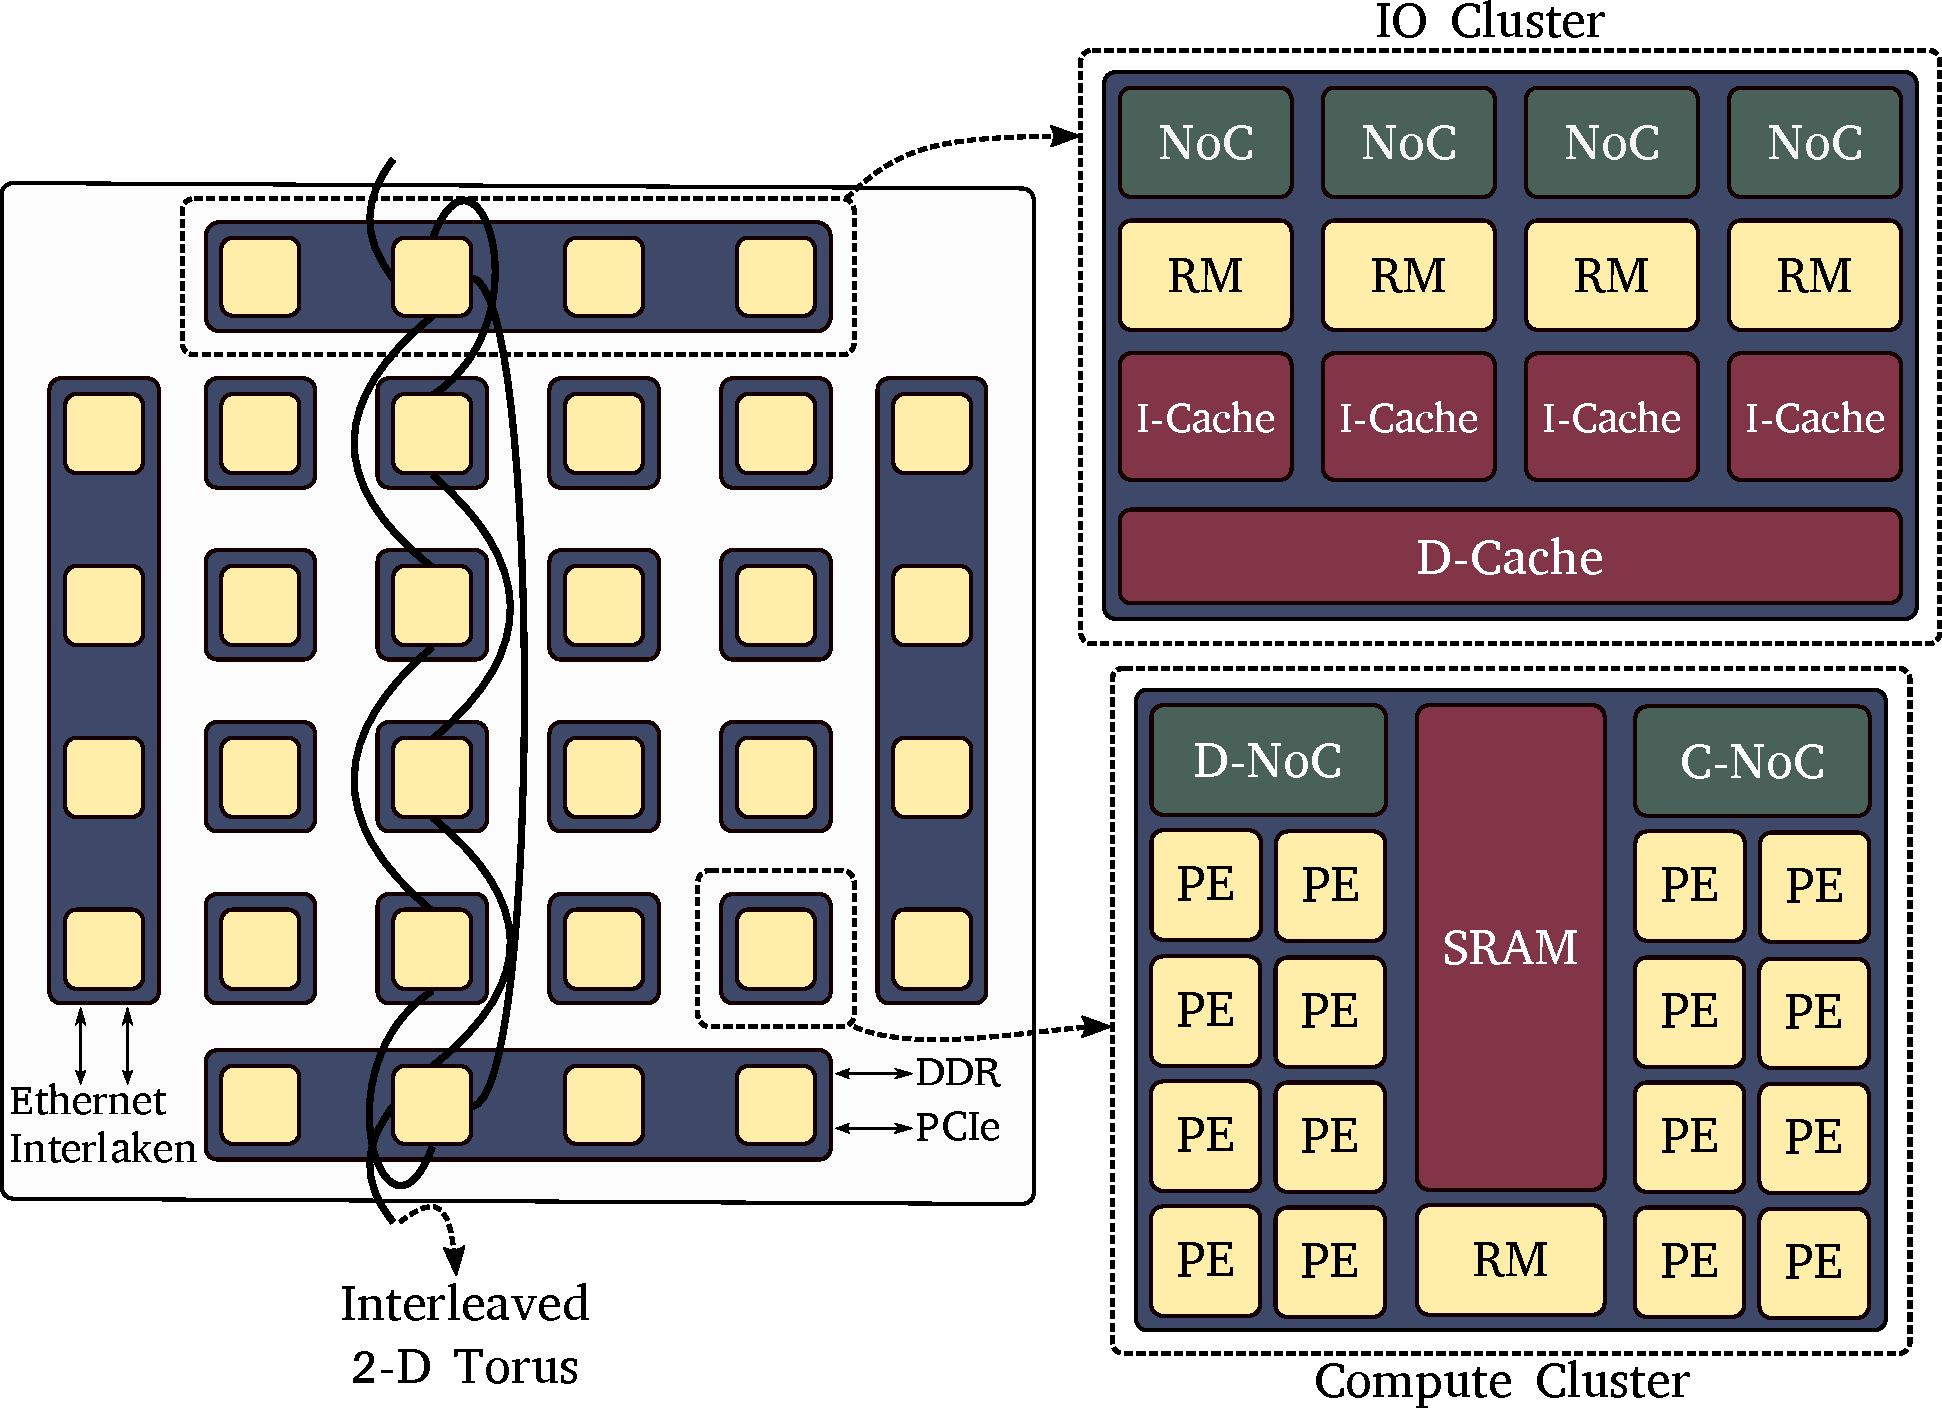
\includegraphics[width=0.90\linewidth]{arch-mppa}
			\caption{\mppa Architecture Overview.}
			\label{fig:mppa}
	\end{figure}



	\section{Results}
\label{sec:results}

	% Methodology
	To assess the costs of creating and waiting for a task, we created
	a synthetic benchmark that write each byte of 16 memory pages, e.g., 64~KB.
	To guarantee 95\% confidence, 50 replications were performed, the first 10
	being discarded to ignore the warm-up period.

	\begin{table}[t]
	\centering
	\caption{Benchmark parameters for experiments.}
	\label{tab:parameters}
	\begin{tabular}{lccc}
	\toprule
			\textbf{Benchmark}   & \textbf{\#Tasks} & \textbf{\#Threads} & \textbf{Memory} \\
			\midrule
			Single Dispatcher    & [1, 29]          & 1                  & 8~KB            \\
			Multiple Dispatchers & [1, 29]          & 14                 & 112~KB          \\
			Threads              & [1, 29]          & [1, 29]            & [8, 232]~KB     \\
			\bottomrule
	\end{tabular}
	\end{table}

	Table~\ref{tab:parameters} shows the application of this benchmark replicated in three
	different scenarios:
	\begin{enumerate*}[label=(\roman*)]
		\item A single dispatcher handle all tasks sequentially;
		\item Each free slave core contains a different dispatcher serving
			tasks in parallel, resulting in 14 dispatchers;
		\item One thread for each task, ranging from 1 to 29 threads.
	\end{enumerate*}
	The number of tasks was limited to the possible number of simultaneous
	threads within the microkernel not replicate the behavior of tasks in user
	threads. The amount of tasks and threads involved defines into the amount
	of memory required to execute each scenario, where each thread uses 8~KB
	for the stacks. Based on this, we can discern that much no extra effort,
	the user can use task abstraction with dispatchers and keep the amount of
	memory used controlled.

	% Time
	Figure~\ref{fig:time} shows the execution time in $\mu$s for each scenario.
	The times collected are made up of the dispatch/create and wait/join period
	of a task/thread.  Comparing the execution of a single task, the use of
	only one dispatcher showed superior performance to the other scenarios
	because there is no competition for the consumption of tasks, exploring the
	location of the data, and do not require the cost of the creation of a new
	thread. Between	7 to 13 tasks, all scenarios behaved similarly performance
	because the overhead of thread creation and concurrency were balanced by
	the workload of the single dispatcher. After 14 tasks, it is possible to
	notice an increase in the scenario of threads because from that moment,
	there are more threads than cores and they start to compete for execution
	time. In contrast, the scenario with 14 dispatchers showed a lower
	execution time because it needs less time to dispatch and consume a task
	than to create a thread. The single dispatcher scenario has steadily
	increased because the tasks are of regular size. Considering that the tasks
	are of regular size, share memory pages, and are executed in dedicated
	cores, the proposed mechanism showed performance similar to the scenario
	that uses specific threads per task.

	\begin{figure}[t]
			\centering
			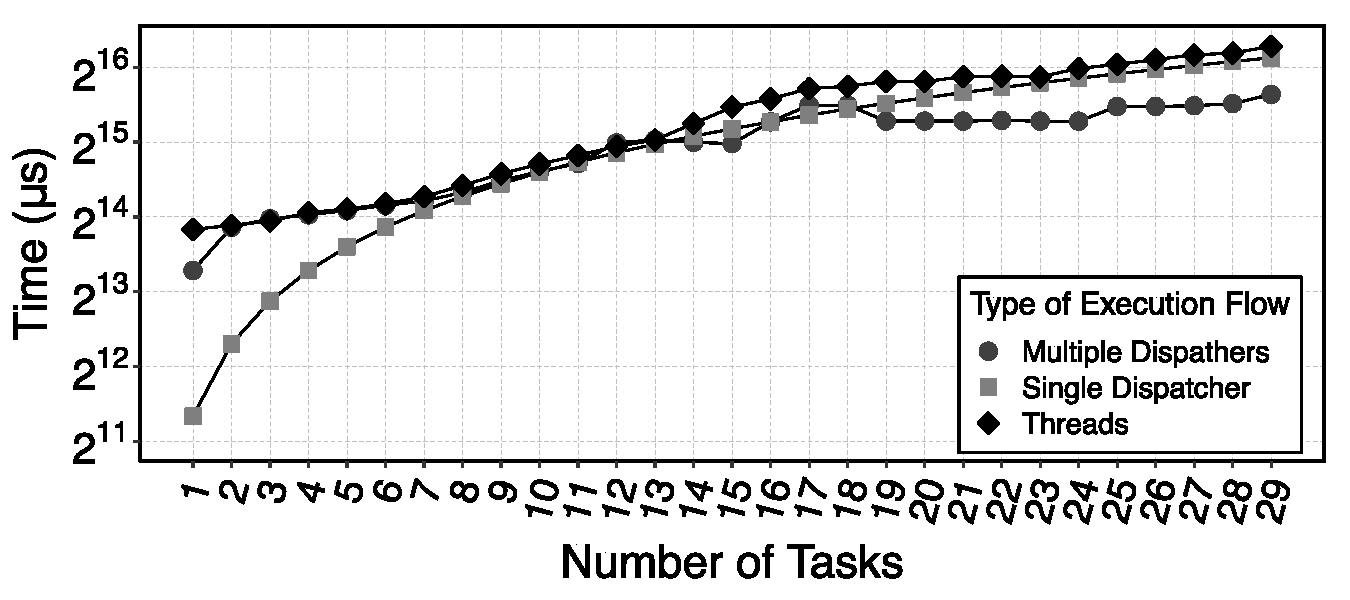
\includegraphics[width=0.97\linewidth]{tasks-time}
			\caption{Runtime Results.}
			\label{fig:time}
	\end{figure}

	\section{Conclusions}
\label{sec:conclusions}

	\lipsum[2-4]


	\bibliography{aux/references.bib}

\end{document}
